\section{Auswertung}
\label{sec:Auswertung}
Zur Berechnung des Mittelwerts $\overline{x}$ einer Größe mit $n$ Messungen der Größe $x$ wird die Formel 
\begin{equation}
  \overline{x}=\frac{1}{n}\sum_{i=1}^n x_n,
  \label{eq:Mittelwert}
\end{equation} verwendet.
Die dazu gehörige Standardabweichung $\sigma$ ergibt sich über 
\begin{equation}
  \sigma=\sqrt{\frac{1}{n-1}\sum_{i=1}^n(x_n-\overline{x})^2}
  \label{eq:Standardabweichung}
\end{equation}
Zum Berechnen der Fehler wird die Gaußsche Fehlerfortpflanzung genutzt 
\begin{equation}
\increment f=\sqrt{\sum_{k=1}^{n}\biggl(\frac{\partial f}{\partial x_\text{k}}\biggr)^2(\increment x_\text{k})^2}\,.
\label{eq:gauss}
\end{equation}
Dabei ist $f$ die zur Berechnung der Größe gegebene Formel und $x_k$ dessen Argumente.
$\increment x_k$ ist der jeweilige Fehler der einzelnen Argumente.
Zunächst wird aus den Messwerten die Winkelrichtgröße $D$ bestimmt.
\begin{table}[H]
  \centering
  \caption{Messwerte zur Bestimmung der Winkelrichtgröße}
  \label{tab:Winkelrichtgroesse}
  \begin{tabular}{
  c c
  }
    \toprule
     $\phi \, / \unit{°}$ & $F\, / \unit{\newton}$\\
    \midrule
    110 & 0.21 \\
    100 & 0.19 \\
    90  & 0.188\\
    80  & 0.168\\
    70  & 0.147\\
    60  & 0.118\\
    50  & 0.090\\
    40  & 0.060\\
    30  & 0.038\\
    20  & 0.016\\
    \bottomrule
  \end{tabular}
\end{table}
Hierfür werden die Drehwinkel $\phi$ zu nächst von $^\circ$ in $rad$ umgerechnet, 
was mit $\phi_\text{neu} = \sfrac{\phi \pi}{180}$ durchgeführt wird.
$D$ wird daraufhin mittels
\begin{equation}
  D = \frac{F R}{\phi_\text{neu}}
\end{equation}
bestimmt.
Dabei ist $F$ die gemessene Kraft und $R$ der Radius, an dem der Kraftmesser befestigt wird.
In diesem Versuch wird $R = \SI{0.2}{\meter}$ gewählt.
Es werden die Winkelrichtgrößen aller Winkel einzeln ausgerechnet.
Anschließend wird der Mittelwert und die Standartabweichung dieser gebildet und die Winkelgröße
\begin{equation*}
  D = \SI{0.01997 \pm 0.00466}{\N \meter}
\end{equation*}
ergibt sich.

Zur Auswertung der Daten in Tabelle \ref{tab:Traegheitsmoment},

\begin{table}[H]
  \centering
  \caption{Messwerte zur Bestimmung des Trägheitsmoments}
  \label{tab:Traegheitsmoment}
  \begin{tabular}{
  c c
  }
    \toprule
     $R \, / \unit{\meter}$ & $F\, / \unit{\newton}$\\
    \midrule
    0.05  & 14.16 \\
    0.075 & 15.97 \\
    0.10  & 18.34 \\
    0.125 & 20.78 \\
    0.15  & 23.47 \\
    0.175 & 26.47 \\
    0.20  & 29.81 \\
    0.225 & 32.81 \\
    0.25  & 35.82 \\
    0.30  & 41.79 \\
    \bottomrule
  \end{tabular}
\end{table}
\begin{figure}[H]
  \centering
  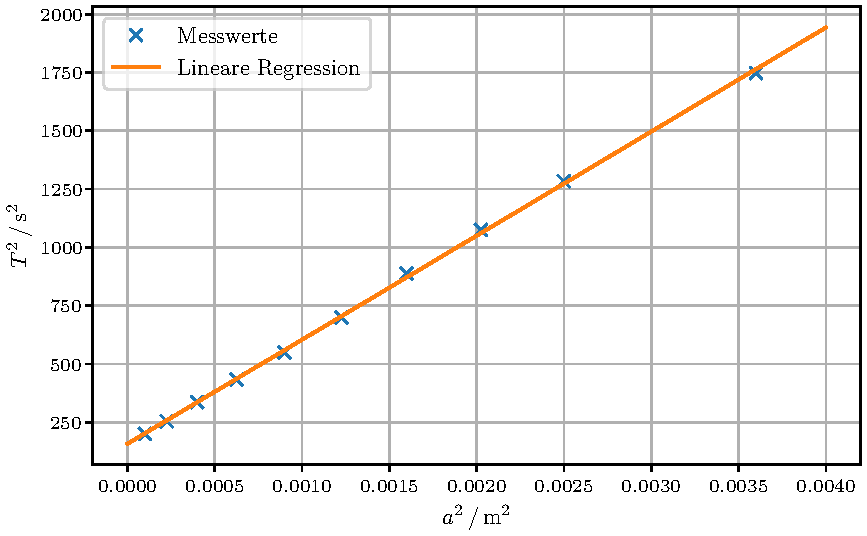
\includegraphics[scale=0.6]{plotI_D.pdf}
  \caption{Das Quadrat des Abstandes aufgetragen gegen das Quadrat der einfachen Schwingungsdauer.}
  \label{fig:Plot1}
\end{figure}



\begin{table}[H]
  \centering
  \caption{5-fache Schwingungsdauer einer Kugel und einers Zylinders}
  \label{tab:Kugel_Zylinder}
  \begin{tabular}{
  c c
  }
    \toprule
     $T_\text{Kugel}\, / \unit{\second}$ & $T_\text{Zylinder}\, / \unit{\second}$\\
    \midrule
    9.15 & 9.47 \\
    9.31 & 9.43 \\
    9.19 & 9.31 \\
    9.34 & 9.47 \\
    9.28 & 9.31 \\
    9.35 & 9.28 \\
    9.41 & 9.41 \\
    9.28 & 9.31 \\
    9.31 & 9.28 \\
    9.35 & 9.28 \\
    \bottomrule
  \end{tabular}
\end{table}
\subsection{Trägheitsmoment einer Kugel}


\begin{table}[H]
  \centering
  \caption{Schwingungsdauer einer Kugel für eine Auslenkung von $90°$.}
  \label{tab:Kugel}
    \begin{tblr}{
      colspec={c|c}
      }
    \toprule
    $t$ / s & $t$ / s\\
    \midrule
    1.83 & 1.87\\
    1.86 & 1.88\\
    1.84 & 1.86\\
    1.87 & 1.86\\
    1.86 & 1.87\\
    \bottomrule
    \end{tblr}
\end{table}
Die verwendete Holzkugel hat die Masse $M_\text{K}=\SI{1172.6}{\gram}$ und den Radius $R_\text{K}=\SI{7.34}{\centi\meter}$. 
Mittels Gl. \eqref{eq:Mittelwert} und \eqref{eq:Standardabweichung} ergibt sich aus den Daten der Tabelle \ref{tab:Kugel} 
eine mittlere Schwingungsdauer von $\overline{t}=\SI{1.86\pm0.015}{\second}$.Mit Einsetzen der gemessenen Werte in Gleichung 
\eqref{eq:Kugel} ein ergibt sich ein Theoriewert für das Trägheitsmoment der Kugel von $I_{\text{K,theo}}=\SI{2.53e-4}
{\kilo\gram\meter\squared}$.
Unter Verwendung der Gl. \eqref{eq:Schwingungsdauer} umgestellt nach $I$ ergibt sich
ein experimenteller Wert von $I=\SI{0.161}{\kilo\gram\meter\squared}$.
\subsection{Trägheitsmoment einer Puppe}
Um das Trägheitsmoment einer Puppe zu bestimmen, muss diese vermessen werden. Wie in der Durchführung bereits 
beschrieben, wurde die Höhe der einzelnen Körperteile jeweils ein mal, die Dicke 5 oder 10 mal gemessen. Folgende 
Maße wurden abgenommen. Die Puppe hat eine Masse von $m_\text{P}=\SI{167.2}{\gram}$.
\begin{table}
  \centering
  \caption{Maße der Puppe.}
  \label{tab:Puppe}
  \begin{tblr}{
    colspec ={c c || c c || c c || c}
  }
  \toprule
    $d_{\text{Bein}}$ / mm  & $d_{\text{B}}$ / mm  & $d_\text{Arm}$ / mm
    & $d_\text{A}$ / mm & $d_\text{Torso}$ / mm & $d_\text{T}$ / mm & $d_\text{Kopf}$ / mm\\
    \midrule
    13,04 & 16,00 & 11,84 & 13,04 & 32,96 & 26,08 & 22,56\\
    13,24 & 16,78 & 11,18 & 12,88 & 37,56 & 31,08 & 27,36\\
    14,32 & 19,42 & 12,46 & 13,24 & 38,74 & 36,08 & 28,44\\
    16,58 & 18,54 & 14,42 & 14,32 & 33,34 & 39,22 & 27,86\\
    17,00 & 16,68 & 14,52 & 13,14 & 25,10 & 40,37 & 24,82\\
    \bottomrule
  \end{tblr}
\end{table}
Die zu den Abmessungen der Puppe in Tabelle \ref{tab:Puppe} gehörigen 
Höhen $H$ der Körperteile wurden jeweils einfach vermessen.
\begin{align*}
  H_\text{A}&=\SI{133.12}{\milli\meter}\\
  H_\text{B}&=\SI{136.58}{\milli\meter}\\
  H_\text{T}&=\SI{99.02}{\milli\meter}\\
  H_\text{K}&=\SI{42.02}{\milli\meter}
\end{align*}
Ziel ist es, über die Volumina der einzelnen Körperteile und die Gesamtmasse 
einzelne Massenwerte zu errechnen. Damit kann der Satz von Steiner angewandt und gezeigt werden.
Mittels Gleichung \eqref{eq:Mittelwert} und Gleichung \eqref{eq:Standardabweichung} erhält werden 
die Mittelwerte und Standardabweichungen der verschiedenen
Dicken berechnet. Das Ergebnis geteilt durch zwei ergibt dies dann den Radius $r$. 
\begin{align*}
  r_\text{A}= \SI{6.6\pm0.5}{\milli\meter}\\
  r_\text{B}= \SI{8.1\pm1.0}{\milli\meter}\\
  r_\text{T}= \SI{17.0\pm2.5}{\milli\meter}\\
  r_\text{K}= \SI{13.1\pm1.1}{\milli\meter}\\
\end{align*}
Das Volumen eines Zylinders ist gegeben durch $V=\pi\cdot r^2\cdot H$. Durch Anwendung der Gauß'schen Fehlerfortpflanzung nach Gl. \eqref{eq:gauss}
ergeben sich für die Volumina sowie deren Fehler 
\begin{align*}
  V_A&=\SI{1.8(0.29)e4}{\milli\meter\cubed},\\
  V_B&=\SI{2.8(0.7)e4} {\milli\meter\cubed},\\
  V_T&=\SI{9.0(2.7)e4} {\milli\meter\cubed},\\
  V_K&=\SI{2.3(0.4)e4} {\milli\meter\cubed}.
\end{align*}
Durch addieren der Volumina sowie verdoppeln des Volumens für Arme und Beine 
wird das Gesamtvolumen bestimmt. Der Fehler ergibt sich aus der Gauß'schen Fehlerfortpflanzung.
\begin{equation*}
  V_\text{Ges}=\qty{2,05+-0,31e5}{\milli\meter\cubed}
\end{equation*}
Nun sollen die Massen $m$ der einzelnen Körperteile bestimmt werden. Dazu wird bestimmt, wie viel
ein Körperteil jeweils vom Gesamtvolumen ausmacht und dieser Anteils-Koeffizient dann mit 
der Gesamtmasse multipliziert. Die Dichte des Holzes wird hierfür als konstant angenommen und
Unterschiede in dem Metall-Anteil der Körperteile vernachlässigt.
\begin{align*}
  m_A&=\frac{V_\text{A}}{V_\text{Ges}}\cdot m_\text{P}=\qty{14.7+-2.9}{\gram}\\
  m_B&=\frac{V_\text{B}}{V_\text{Ges}}\cdot m_\text{P}=\qty{23+-5}{\gram}\\
  m_T&=\frac{V_\text{T}}{V_\text{Ges}}\cdot m_\text{P}=\qty{74+-14}{\gram}\\
  m_K&=\frac{V_\text{K}}{V_\text{Ges}}\cdot m_\text{P}=\qty{19+-4}{\gram}
\end{align*}
  Die Fehler ergeben sich erneut über Gauß'sche Fehlerfortpflanzung \eqref{eq:gauss}.
Nun soll der Satz von Steiner \eqref{eq:Steiner} angewandt bzw. überprüft werden.
anhand zwei verschiedener Sitzpositionden einer Puppe überprüft werden. Mit seitlich ausgestreckten
Armen im 90°-Winkel zum Oberkörper und geraden Beinen befindet sich die Puppe im 1. Zustand. werden 
zusätzlich noch die Beine, ebenfalls in einem 90°-Winkel zum Oberkörper, ausgestreckt.
Dazu werden mittels \eqref{eq:Steiner} die einzelnen Trägheitsmomente ermittelt.
Für die Beine, den Kopf und den Torso wird angenommen, dass die Drehachse durch den Schwerpunkt
verläuft. Die Beine werden als ein Zylinder mit Radius $r=D_\text{B}=2r_\text{B}$ angenommen. Der Kopf und Torso werden
jeweils als auch als Zylinder angenommen. Das Trägheitsmoment der Arme wird mithilfe der Formel in Gl. 
\eqref{eq:falscher_zylinder} berechnet. Die Verschiebung $a$ zwischen Dreh- und Schwerpunktsachse setzt 
sich aus dem Radius des Torsos und der Länge des Arms zusammen.
\begin{align*}
  a&=r_T+\frac{H_\text{A}}{2}
\intertext{Damit ergibt sich für einen Arm mit Gl.\eqref{eq:Steiner}}
\label{eq:Arme}
I_\text{A}&=m_\text{A}\left(\frac{r_\text{A}^2}{4}+\frac{(r_T*0,5*H_\text{A})^2}{12}\right)\,,
\intertext{Für das Trägheitsmoment der Beine ergibt sich nach Gl. \eqref{eq:Zylinder}}
I_\text{2B}&=\frac{2m_\text{B}\cdot 2r_\text{B}^2}{2}=m_\text{B}\cdot r_\text{B}^2\,.
\intertext{Analog dazu für Kopf und Torso}
I_\text{i}&=\frac{m_i\cdot r_i^2}{2};\quad i\in\{T,K\}\,.
\end{align*}
Aus diesen Formeln und vorher berechneten Werten ergibt sich
der Theorie-Wert für das Gesamträgheitsmoment
\begin{equation}
  I_\text{1,theo}=\qty{32.1+-6.8e-4}{\kilo\gram\meter\squared}\,.
\end{equation}0.0032185662+/-0.0006804836
Das Trägheitsmoment soll nun mittels Gleichung \eqref{eq:Schwingungsdauer} und den in Tabelle
\ref{tab:Zeiten1_Puppe} aufgeführten Daten bestimmt und mit dem Theorie-Wert abgeglichen werden.
Gl. \eqref{eq:Schwingungsdauer} nach $I$ umgestellt ergibt
\begin{equation}
  I=\frac{T^2}{2\pi}D\,.
  \label{eq:Traegheitsmoment}
\end{equation}
\begin{table}
  \centering
  \caption{Messdaten der Schwingungsdauer für zwei verschiedene Winkel in 
  der ersten Körperhaltung der Puppe.}
  \label{tab:Zeiten1_Puppe}
  \begin{tblr}{colspec={S S},
    row{1}={guard}, row{2}={guard},
    }
    \toprule
    $\phi=\qty{90}{\degree}$ & $\phi=\qty{120}{\degree}$\\
    $5T$ / s & $5T$ / s\\
    \midrule
    3,06 & 2,88 \\
    3,28 & 2,87 \\
    2,72 & 2,87 \\
    3,06 & 2,84 \\
    3,16 & 2,90 \\
    \bottomrule
  \end{tblr}
\end{table}
FÜr das experimentell bestimmte Trägheitsmoment der Puppe in der ersten Haltung ergibt sich 
\begin{equation*}
  I_\text{1,exp}=\qty{11,2+-02,9e-4}{\kilo\gram\meter\squared}
\end{equation*}
Für die zweite Haltung der Puppe verläuft die Rechnung sehr analog. Die Trägheitsmomente der Arme, des Torsos 
sowie des Kopfes können übernommen werden, die Beine müssen jedoch mittels des Satzes von Steiner berechnet werden.
Dies geschieht jedoch genau wie bei der anderen Haltung für die Arme mit Gleichung\eqref{eq:Arme} und \eqref{eq:Steiner}.
Die Beine werden ebenso wieder als ein Zylinder mit doppeltem Radius angenommen.
Es ergibt sich ein gesamt theoretisch bestimmtes Trägheitsmoment 
\begin{equation*}
  I_\text{2,theo}=\qty{5,2+-1,3e-3}{\kilo\gram\meter\squared}
\end{equation*}
Mit den in Tabelle \ref{tab:Zeiten2_Puppe} und Gleichung \eqref{eq:Trägheitsmoment} ergibt sich
ein experimentell bestimmtes Trägheitsmoment 
\begin{equation*}
  I_\text{2,exp}=\qty{3+-0,73e-3}{\kilo\gram\meter\squared}\,.
\end{equation*}
\begin{table}
  \centering
  \caption{Messdaten der Schwingungsdauer für zwei verschiedene Winkel in 
  der zweiten Körperhaltung der Puppe.}
  \label{tab:Zeiten2_Puppe}
  \begin{tblr}{colspec={S S},
    row{1}={guard}, row{2}={guard},
    }
    \toprule
    $\phi=\qty{90}{\degree}$ & $\phi=\qty{120}{\degree}$\\
    $5T$ / s & $5T$ / s\\
    \midrule
    4,84 & 4,85 \\
    4,87 & 4,94 \\
    4,72 & 4,90 \\
    4,93 & 4,97 \\
    4,79 & 4,94 \\
    \bottomrule
  \end{tblr}
\end{table}
